% !TEX program = xelatex

\documentclass[11pt,oneside]{book}

%%%%%%%%%%%%% Geometry
\usepackage[a4paper,left=2.5cm,right=2.5cm, bottom=2.5cm,top=2.5cm]{geometry}
\usepackage{fontspec}
%%%%%%%%%%%%%%% Insert Code
\usepackage[utf8]{inputenc}
\usepackage{listings}
\usepackage{color}

\definecolor{mygreen}{rgb}{0,0.6,0}
\definecolor{mygray}{rgb}{0.5,0.5,0.5}
\definecolor{mygray2}{rgb}{0.58,0.5,0.82}

\lstset{ %
backgroundcolor=\color{white},   % choose the background color
basicstyle=\footnotesize\ttfamily,     % size of fonts used for the code
columns=fullflexible,
breaklines=true,                 % automatic line breaking only at whitespace
captionpos=b,                    % sets the caption-position to bottom
tabsize=4,
commentstyle=\color{mygreen},    % comment style
escapeinside={\%*}{*)},          % if you want to add LaTeX within your code
keywordstyle=\color{blue},       % keyword style
stringstyle=\color{mygray2}\ttfamily,     % string literal style
frame=single,
rulesepcolor=\color{red!20!green!20!blue!20},
% identifierstyle=\color{red},
language=c++,
}

\usepackage[english]{babel}
\usepackage[palette=munch]{nexus}
\usepackage{ctex} 
%%%%%%%%%%%%%%%% hyperref
\usepackage{lipsum}
\usepackage[verbose]{hyperref}
\hypersetup{ 
    hidelinks
}
\setlength{\XeTeXLinkMargin}{-1pt}

\begin{document}

\pagestyle{empty}

\definecolor{plop}{HTML}{4D7186}
\begin{textblock}{1}(0,0)
    \noindent\textcolor{plop}{\rule{\paperwidth}{.55\paperheight}}
\end{textblock}

\begin{textblock}{1}(0,.55)
    \noindent\textcolor{black}{\rule{\paperwidth}{.45\paperheight}}
\end{textblock}

\begin{textblock}{.45}(.52, .05)
    \begin{center}
        
\includegraphics[width=.4\paperwidth]{logo2.png}
    \end{center}
\end{textblock}

\begin{textblock}{.45}(.53, .12)
    \begin{center}
        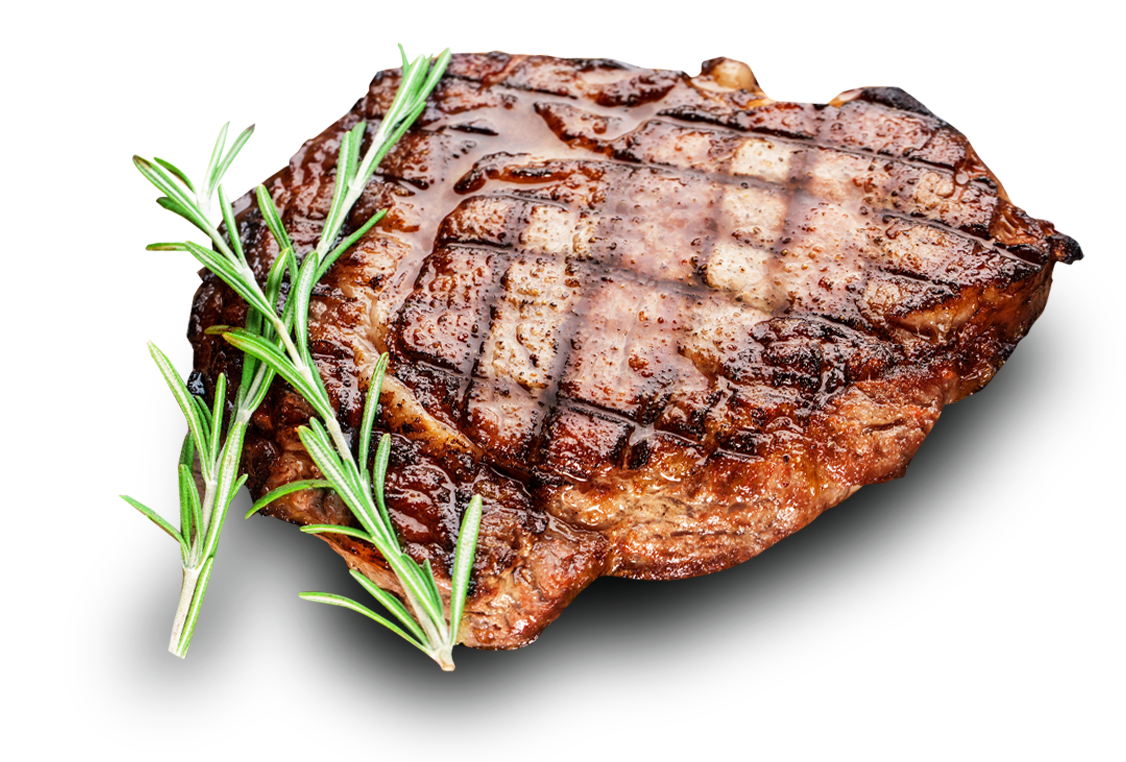
\includegraphics[width=.4\paperwidth]{logo.png}
    \end{center}
\end{textblock}


\begin{textblock}{1}(.1, .09)
    \noindent{\fontsize{64.02}{2}\selectfont
        \bfseries\textcolor{white}{知识之书 \\ \\ \hspace{1cm} 呓语魔典 \\ \\ \hspace{4cm}印象笔记}}
\end{textblock}

\begin{textblock}{1}(.1, .38)
    \noindent {\fontsize{24.88}{2}\selectfont
    \bfseries\textcolor{white}{对所学所思做一些持久化、去碎片化处理}}
\end{textblock}

% \begin{textblock}{1}(.1,.21)
%     \noindent{\fontsize{30}{2}\selectfont
%         \bfseries\textcolor{white}{for \LaTeX}}
% \end{textblock}

\begin{textblock}{1}(.1,.45)
    \noindent {\fontsize{22.74}{2}\selectfont
        \bfseries\textcolor{white}{吴继鹏 著}}
\end{textblock}



\begin{textblock}{.9}(.05,.56)
    \begin{flushright}
        \noindent {\fontsize{20.74}{2}\selectfont
            \bfseries\textcolor{orange}{version 1.1}}
    \end{flushright}
\end{textblock}



\begin{textblock}{.45}(.5,.82)
    \begin{center}
        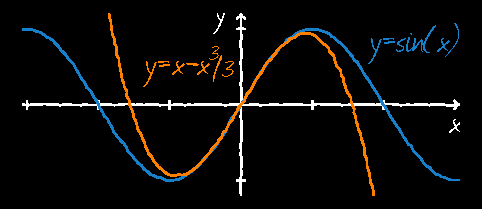
\includegraphics[width=.45\paperwidth]{dlsin}
    \end{center}
\end{textblock}

\begin{textblock}{.4}(.05,.65)
    \begin{center}
        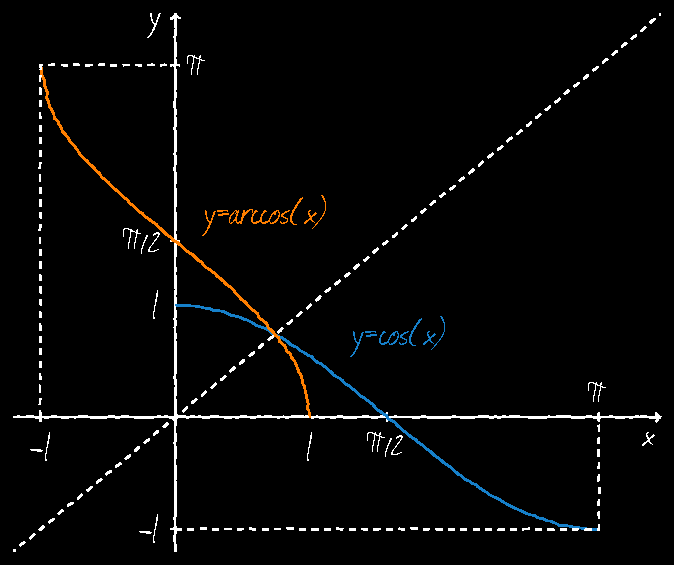
\includegraphics[width=.4\paperwidth]{arccos}
    \end{center}
\end{textblock}


\begin{textblock}{.6}(.05,.6)
    \noindent {\fontsize{20.74}{18}%
    \textcolor{white}{$\displaystyle(a+b)^n = \sum_{k=0}^n 
                \binom{n}{k} a^kb^{n-k}$}}
\end{textblock}


\begin{textblock}{.4}(.4,.77)
    \noindent {\fontsize{17.28}{18}%
    \textcolor{white!80}{$\displaystyle 
                \neg (p\vee q) \equiv (\neg p)\wedge (\neg q)$}}
\end{textblock}

\begin{textblock}{.4}(.1,.93)
    \noindent {\fontsize{14.4}{18}%
    \textcolor{white!50}{$\displaystyle 
                \binom{n}{k} = \frac{n!}{k!(n-k)!}$}}
\end{textblock}


\begin{textblock}{.6}(.5,.69)
    \noindent {\fontsize{17.28}{18}%
    \textcolor{white!10}{$\displaystyle 
                \zeta_k = |a|^{1/n} \mathrm{e}^{i(\mathrm{arg}(a)+2k\pi)/n}$}}
\end{textblock}


\begin{textblock}{.3}(.75,.73)
    \noindent {\fontsize{17.28}{18}%
    \textcolor{white!10}{$\displaystyle \mathrm{e}^{i\pi}+1=0$}}
\end{textblock}



\null\newpage\pagestyle{nexus}

\tableofcontents

%%%%%%%%%%%%%%%%%%%%%%%
\chapter{现代C++}
\section{语言与范式}
\subsection{默认采用\{\}初始化}
现代C++变量的初始化应该优先用\{\},完美兼容所有类型的变量。
这么做并不是特别必要,但是有一种麦克斯韦光、电、磁统一的美感。

\begin{lstlisting}[language=C++]
    std::vector<int> v{ 1, 3, 5 }; 
\end{lstlisting}

\begin{lstlisting}[language=C++]
    double x, y, z;
    int sum1{ x + y + z }; // 报错,一定要是int!
    int sum2(x + y + z); // okay,隐式转成int了!
    int sum3 = x + y + z; // 同上!
\end{lstlisting}

\begin{lstlisting}[language=C++]
    Widget w2(); // 定义了一个函数,雪崩!
    Widget w2{}; // 调用ctor舒适化!
\end{lstlisting}

类对象要注意,如果存在参数为initializer list的ctor,则\{\}初始化必然会优先调这个ctor,没有才会调普通ctor。所以自己写的代码干脆禁用initializer list,免得它劫持\{\}初始化,给人造成误解。vector里就定义了initializer list,使得()与\{\}相同参数初始化意义不同!

\begin{lstlisting}[language=C++]
std::vector<int> v1(10, 20); // 创建10个值为20的元素
std::vector<int> v2{10, 20}; // 创建两个元素:10, 20
\end{lstlisting}


\subsection{使用alias,不用typedef}

下面这种写起来长度差不多。
\begin{lstlisting}[language=C++]
typedef void (*FP)(int, const std::string&); // typedef
using FP = void (*)(int, const std::string&); // alias
\end{lstlisting}

但涉及template时,typedef根本不支持,要耍一个花招,加一层struct做包装。
\begin{lstlisting}[language=C++]
    template<typename T> 
    using MyAllocList = std::list<T, MyAlloc<T>>; 
    MyAllocList<Widget> lw; // client code

    template<typename T> // MyAllocList<T>::type
    struct MyAllocList { 
     typedef std::list<T, MyAlloc<T>> type; 
    }; 
    MyAllocList<Widget>::type lw; // client code
\end{lstlisting}
    


\subsection{使用enum class,少用enum}
\begin{lstlisting}[language=C++]
    enum Color { black, white, red }; // 虽在花括号内,实则定义在外层代码块里。
    auto white = false; // 错了,white已被定义!

    enum class Color { black, white, red }; // 虽在花括号内,实则定义在外层代码块里。
    auto white = false; // 没问题!
    auto c = Color::white; // 正确!
\end{lstlisting}

enum class是强类型enum,有自己的作用域,禁止隐式类型转换,还允许"enum class Color;"这样的前置声明。

此外,enum class内部的默认类型是int,也可以自己设定更合适的类型。
\begin{lstlisting}[language=C++]
    enum class Status: std::uint32_t { 
        good = 0,
        failed = 1,
        incomplete = 100,
        indeterminate = 0xFFFFFFFF
    };
\end{lstlisting}

enum也不是一无是处,有时候专门用来做隐式转换,写起来更简单。
\begin{lstlisting}[language=C++]
    using UserInfo = std::tuple<std::string, std::string,  std::size_t> ; // name, email, reputation
    enum UserInfoFields { name, email, reputation };
    UserInfo uInfo; 
    auto val = std::get<email>(uInfo); // 相当于std::get<1>(uInfo)
\end{lstlisting}

enum class其实也可以做这种转换,需要事先写好constexpr函数方便这种转换。
\begin{lstlisting}[language=C++]
    template<typename E> // C++14
    constexpr auto
    toUType(E enumerator) noexcept
    {
        return static_cast<std::underlying_type_t<E>>(enumerator);
    }
    //还是比enum长,但是避免了namespace污染。
    auto val = std::get<toUType(UserInfoFields::email)>(uInfo);
\end{lstlisting}



\section{多线程编程}
\lipsum[1-2]

\section{深度学习框架}
\lipsum[1-2]

%%%%%%%%%%%%%%%%%%%%%%%
\chapter{算法与数据结构}
\section{数据结构}

\section{Leetcode中的算法}

\section{高级话题中的算法}


\chapter{分布式计算与存储}
\section{kubernetes容器集群}
\lipsum[1-3]

\section{分布式系统的传统实现}
\lipsum[1-2]

\section{KV Store}
\lipsum[1-2]
\subsection{Leveldb}

%%%%%%%%%%%%%%%%%%%%%%%

\chapter{前端}
\section{脚手架与工具链}
\lipsum[1-3]
\section{Stateless模块化编程范式}
\lipsum[1-3]

%%%%%%%%%%%%%%%%%%%%%%%

\chapter{机器学习}
\section{深度学习}
\lipsum[1-3]

\section{传统方法}
\lipsum[1-1]

%%%%%%%%%%%%%%%%%%%%%%%
\chapter{Java以及它的生态}
\section{Java8/9/10新特性}
\lipsum[1-2]
\section{Spring WebFlux}
\lipsum[1-2]
\section{Spring-boot}
\lipsum[1-2]

%%%%%%%%%%%%%%%%%%%%%%%
\chapter{Python后端开发}
\section{语法与语法糖}
\lipsum[1-2]
\section{Flask}
\lipsum[1-2]
\section{Tornado}
\lipsum[1-2]

%%%%%%%%%%%%%%%%%%%%%%%
\chapter{工程经验}
\section{BloodMiser}
\lipsum[1-3]
\section{军用智能计算}
\lipsum[1-3]
\section{Stateless}
\lipsum[1-3]
\section{Do-Not-Yarn}
\lipsum[1-3]

%%%%%%%%%%%%%%%%%%%%%%%
\chapter{社会经验}
\section{职场}
\lipsum[1-3]
\section{生活}
\lipsum[1-3]

%%%%%%%%%%%%%%%%%%%%%%%
\chapter{地缘政治}
\section{中美武器装备}
\lipsum[1-3]
\section{美国国内政治}
\lipsum[1-3]
\section{周边国家与台湾}
\lipsum[1-3]

\end{document}

